\documentclass[10pt]{article}
\usepackage[dutch,english]{babel}
\usepackage[T1]{fontenc}
\usepackage[lining]{libertine}
\usepackage{textcase}
\usepackage{microtype}
\pdfcompresslevel=9
\usepackage{graphicx}
\usepackage{chngpage}
\usepackage{color}

\newcommand{\makenote}[1]{{ \color{red} [#1]}}

\newlength{\mytextwidth}
\setlength{\mytextwidth}{60mm}
\newlength{\mytextheight}
\setlength{\mytextheight}{20cm}
\usepackage[papersize={86mm,236mm}, width=\mytextwidth, height=\mytextheight, hmarginratio={1:1},vmarginratio={1:1},bindingoffset=0mm]{geometry}


\thispagestyle{empty}

\newcommand{\attribute}[1]{\hspace*{1mm}\hfill{\footnotesize\textit{-- #1}}}%
\DeclareRobustCommand{\spacedallcaps}[1]{\textls[160]{\MakeTextUppercase{#1}}}%
\DeclareRobustCommand{\spacedlowsmallcaps}[1]{\textls[80]{\scshape\MakeTextLowercase{#1}}}%

\newlength{\headerspacing}
\setlength{\headerspacing}{3mm}

\linespread{1.05}
\usepackage{enumitem}

\begin{document}
\begin{center}
\vspace*{.2mm}
\large\spacedallcaps{Invitation}\normalsize\\ 
\rule{.5\linewidth}{0.1mm}\\
\vspace{\headerspacing}
For attending the public\\
defense of the PhD thesis
%
\vspace{2\headerspacing}
\begin{adjustwidth}{-1in}{-1in}\begin{center}
\spacedallcaps{Visual Analytics Applied to}\\
\spacedallcaps{Image Analysis}\\
\end{center}\end{adjustwidth}
\begin{adjustwidth}{-1ex}{-1ex}\begin{center}
\small From Segmentation to Classification
\end{center}\end{adjustwidth}
\vspace{\headerspacing}
\small by \normalsize\\
\vspace{\headerspacing}
\spacedlowsmallcaps{Paulo Eduardo Rauber}\\
\vspace{\headerspacing}
20th February 2017 at 16:15 hrs\\
Academiegebouw\\
University of Groningen\\
Broerstraat 5\\
%
\vspace{2\headerspacing}
%
\spacedlowsmallcaps{Reception}\\
\vspace{\headerspacing}
\makenote{Reception date and address}\\
%
\vspace{2\headerspacing}
%
\spacedlowsmallcaps{Paranymphs}\\
\vspace{\headerspacing}
\makenote{Paranymph name}\\
\small \makenote{Paranymph e-mail} \normalsize \\
\vspace{\headerspacing}
\makenote{Paranymph name}\\
\small \makenote{Paranymph e-mail}

\begin{figure}[b]
\centering
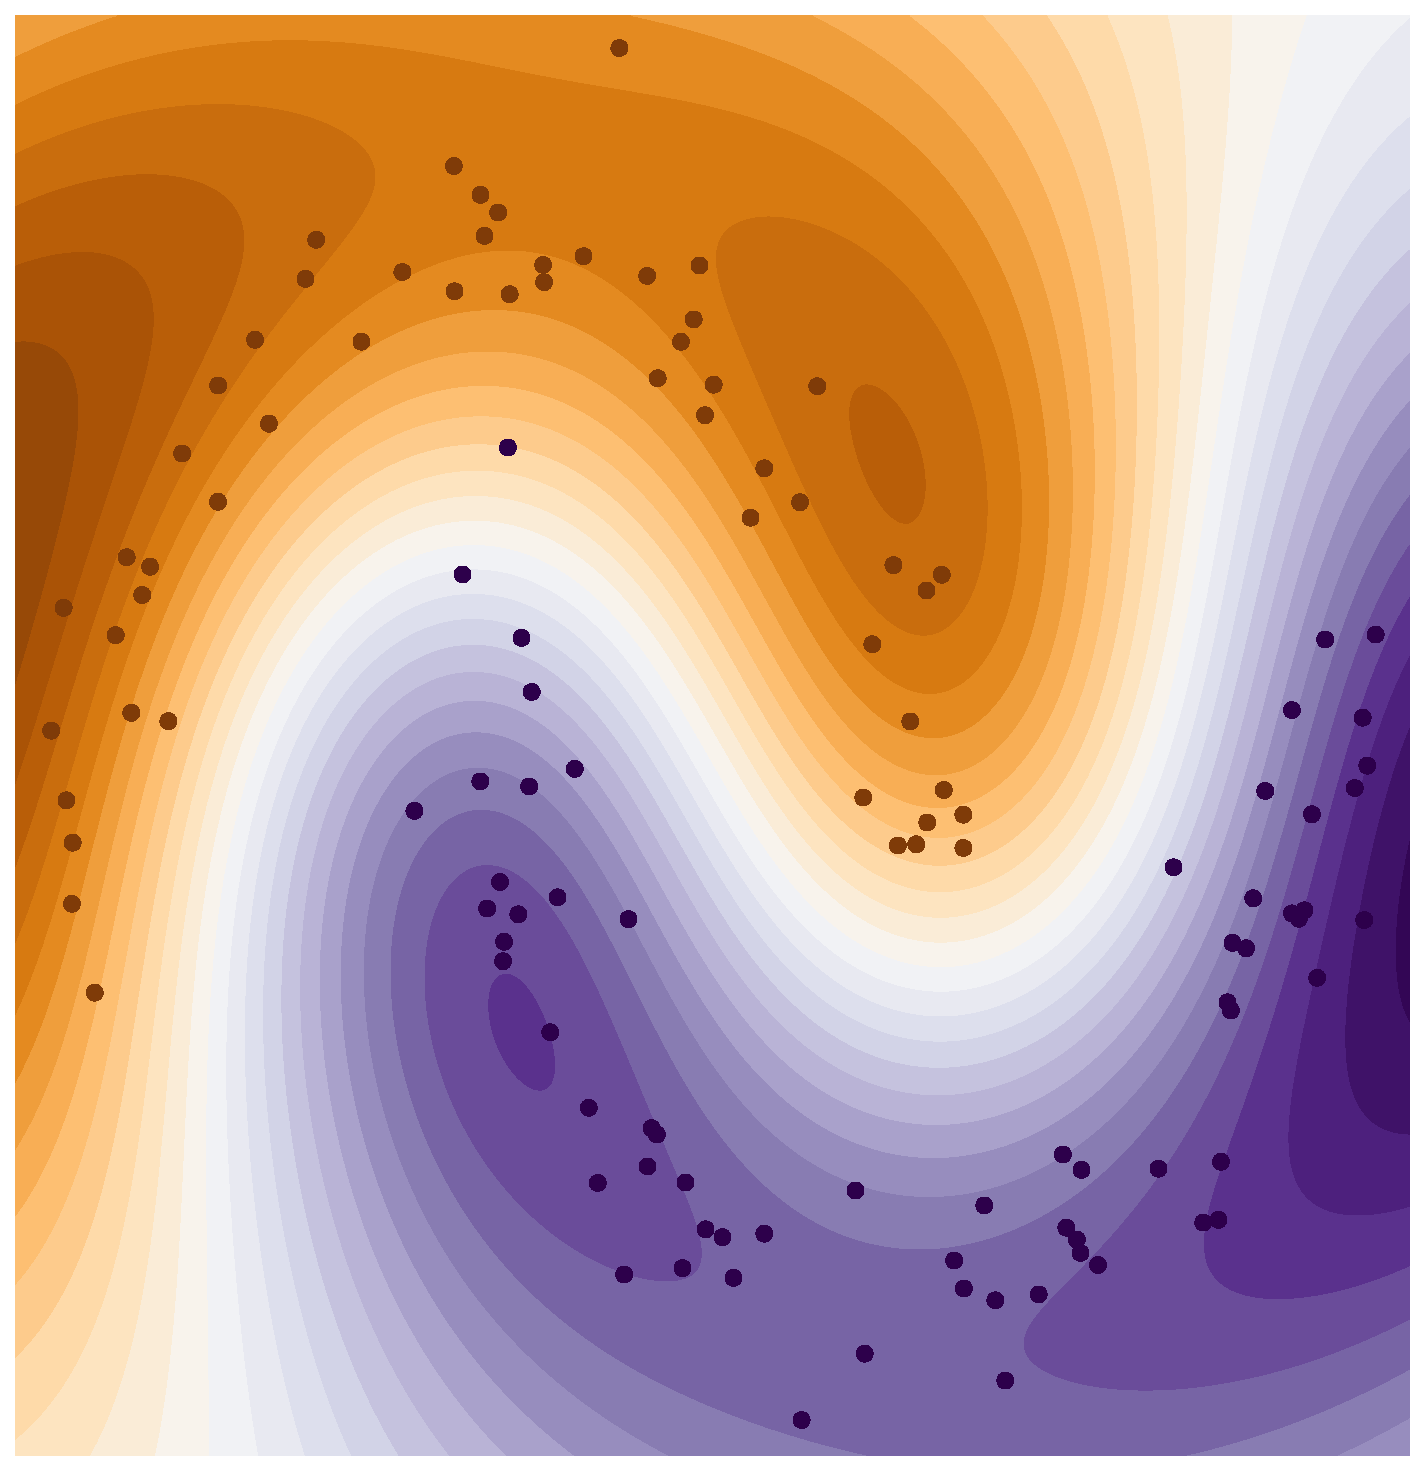
\includegraphics[width=0.8\textwidth]{figures/cover_graphic.eps}
\end{figure} 

\end{center}
\end{document}
